

\documentclass[a4paper,12pt,spanish]{article}

\usepackage[utf8]{inputenc}


\usepackage{blindtext}
%\usepackage{microtype}
\usepackage{amsfonts, amsmath, amsthm, amssymb}
%\usepackage{fancyhdr}
%\usepackage{index}
%\usepackage{multicol}    

\usepackage[T1]{fontenc}
\usepackage[utf8]{inputenc}
\usepackage{graphicx}
\usepackage[spanish,es-tabla]{babel}
\usepackage{url}
\usepackage{enumitem}

\usepackage[unicode=true, pdfusetitle,
bookmarks=true,bookmarksnumbered=false,bookmarksopen=false,
breaklinks=true,pdfborder={0 0 1},backref=false,colorlinks=false]
{hyperref}

\usepackage{listings}


\usepackage{siunitx} %para el sistema internacional
\usepackage[export]{adjustbox}
\usepackage{booktabs} 
\usepackage{subcaption}

\usepackage{float}


\newcommand{\address}[1]{
	\par {\raggedright #1
		\vspace{1.4em}
		\noindent\par}
}


\pagenumbering{gobble}
\include{noNumberPage}
\pagenumbering{arabic}
\setcounter{page}{78}

%tutorial de tablas latex: https://manualdelatex.com/tutoriales/tablas

\usepackage{multirow}

% \usepackage[table,xcdraw]{xcolor}


%Inicio del documento (hasta que se cierre con \end{document}
\begin{document}
	
	
	
	
	
	\title{El transistor bipolar}
	
	%\author{Adrián Rivero Fernández}
	\date{}
	
	\maketitle
	
	
	
\begin{abstract} %resumen
	En esta práctica, identificaremos los terminales del transistor (emisor, base y colector) y estudiaremos sus tres zonas de trabajo (corte, activa y saturación).
	
	\begin{itemize}
		\item Calcularemos el factor $\beta$ del transistor e identificaremos sus zonas de trabajo.
		\item Obtendremos las curvas características $I_C$-$V_CE$ para diferentes corrientes de base.
		\item Calcularemos diferentes sistemas de polarización del transistor.
	\end{itemize}
\end{abstract}
	

\section{Introducción}

El transistor bipolar se compone de dos uniones PN contrapuestas. Son tres regiones semiconductoras llamadas emisor, base y colector. 

Existen transistores NPN y PNP, como vemos en la Figura 1. 

\begin{figure}[H]
	\centering
	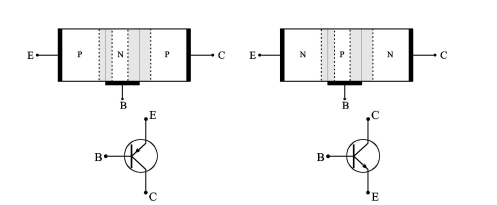
\includegraphics[width=1.1\linewidth]{Figura1}
	\caption{Transistor bipolar PNP (izquierda) y NPN (derecha)}
	\label{fig:figura1}
\end{figure}

En esta práctica nos centramos en el NPN, aunque el comportamiento de los PNP es análogo.


El emisor en un transistor NPN es la zona más fuertemente
dopada con donadores de electrones, y tiene un ancho intermedio entre el de la base y el colector. Su función es la de emitir electrones a la base. La base es la zona más estrecha y se está débilmente dopada con aceptores
de electrones. El colector es la zona más ancha, y se encuentra dopado con donadores de electrones en cantidad intermedia entre el emisor y la base.

Las condiciones normales de funcionamiento de un transistor NPN se dan cuando el diodo B-E se encuentra polarizado en directa ($V_{BE} = 0,7 \si{V}$) y el diodo B-C se encuentra polarizado en inversa.
En esta situación gran parte de los electrones que fluyen del emisor a la base consiguen atravesarla, debido a su poco grosor y débil dopado, y llegar al colector.

El transistor tiene tres zonas de funcionamiento:\\

\textbf{Zona de saturación: } El colector está directamente polarizado, el transistor se comporta como una pequeña resistencia de caída de tensión $V_{CE}\approxeq 0,3 \si{V}$. Aumentar la corriente de base no provoca un aumento de la corriente de colector, ya que esta depende solo de la tensión entre emisor y colector. Funciona como un interrupor cerrado entre emisor-colector.

\textbf{Zona activa:} se comporta como una fuente de corriente controlada por la corriente de la base. Con pequeños aumentos de la corriente de base la corriente de colector aumenta notablemente, casi de forma independiente de la tensión entre emisor-colector. El diodo B-E debe estar polarizado directamente y el B-C inversamente.

\textbf{Zona de corte:} ambas uniones polarizadas inversamente. La corriente de base es nula, y equivale a mantener el circuito base-emisorr abierto. La corriente de colector es casi nula y se puede considerar el circuito C-E como un circuito abierto.\\

Cuando los transistores se usan como amplificadores de señal es usan en la zona activa. Las zonas de corte y saturación se usan para circuitos digitales.


\section{Material y métodos}

Utilizaremos resistencias comerciales de distintos valores, un transistor bipolar de pequeña señal 2N3904, una fuente de alimentación de salida variable (0-12V) y fija de $\pm$ 5V, una pila de 9V, un polímetro para tomar las mediciones, y una placa de prototipo protoboard donde montar el circuito.

\subsection{Zonas de funcionamiento del transistor bipolar}

Identificamos los terminales del transistor y montamos el circuito de la Figura 2, con la fuente $V_{CC}$ a 5V y variando la fuente de tensión $V_{BB}$ entre 0 y 12V, midiendo los valores del potencial en las resistencias, $V_{RB}$ y $V_{RC}$. A partir de los datos, calcular las corrientes de base y de colector, y el voltaje $V_{CE}$ para cada punto.

Organizaremos todo eso en una tabla y representaremos en una gráfica la corriente del colector frente a la corriente de base, e identificaremos las zonas de trabajo.


\begin{figure}[H]
	\centering
	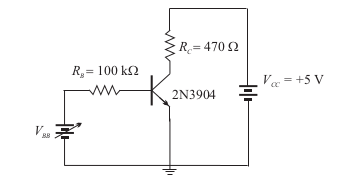
\includegraphics[width=0.7\linewidth]{circuito}
	\caption{circuito a montar}
	\label{fig:circuito}
\end{figure}



\subsection{Curvas características $I_C - V_{CC}$ para diferentes valores de la corriente de base}

Fijando la tensión $V_{BB}$ a 5V, variaremos la tensión $V_{CC}$ entre 0,3V y 12V y mediremos para cada voltaje $V_{CC}$, el voltaje que cae en $R_B$, en $R_C$ y $V_{CE}$. 
Representaremos en una gráfica $I_C$ frente a $V_{CC}$.

Repetiremos lo anterior con una tensión de $V_{BB}= 9 \si{V}$.

\subsection{Diferentes circuitos de polarización del transistor}

Implementaremos diferentes circuitos de polarización del transistor en la zona activa y en la configuración de emisor común. Determinaremos teóricamente los valores de las resistencias necesarias para obtener el punto de polarización determinado por los datos de la última parte del primer apartado para la corriente de colector $V_{CE}$ y $\beta$.

Después, construiremos cada circuito y determinaremos los valores experimentales.


\section{Resultados y discusión}

\subsection{Zonas de funcionamiento del transistor bipolar}

La Tabla 1 recoge los valores medidos y calculados. En la Figura 3 tenemos la gráfica que representa la corriente de colector frente a la corriente de base.



\begin{table}[H]
	\centering
	\begin{tabular}{|c|c|c|c|c|c|}
		\hline
		$V_{BB}$ (V) & $V_{RB}$ (V)   & $I_B$ (A)     & $V_{RC}$ (V)  & $I_C$ (A)    & $V_{CE}$ (V)  \\ 
		&[$\pm0,001$] &[$\pm1$E-08] &[$\pm0,001$] &[$\pm2$E-06]  &[$\pm0,001$]\\\hline
		0,3   & 0,001 & 5E-09     & 0      &   0     & 5      \\ \hline
		0,6   & 0,008 & 8,1E-08   & 0,0055 &  1,17E-05 & 4,9945 \\ \hline
		0,9   & 0,321  & 3,21E-06  & 0,241  & 0,000512  & 4,759  \\ \hline
		1,2   & 0,55   & 5,5E-06   & 0,433  & 0,000921  & 4,567  \\ \hline
		1,5   & 0,8    & 8E-06     & 0,685  & 0,001457  & 4,315  \\ \hline
		2     & 1,352  & 1,352E-05 & 1,089  & 0,002317  & 3,911  \\ \hline
		2,5   & 1,893  & 1,893E-05 & 1,535  & 0,003266  & 3,465  \\ \hline
		3     & 2,353  & 2,353E-05 & 1,936  & 0,004119  & 3,064  \\ \hline
		3,5   & 2,893  & 2,893E-05 & 2,361  & 0,005023  & 2,639  \\ \hline
		4     & 3,384  & 3,384E-05 & 2,762  & 0,005877  & 2,238  \\ \hline
		4,5   & 3,816  & 3,816E-05 & 3,112  & 0,006621  & 1,888  \\ \hline
		5     & 4,33   & 4,33E-05  & 3,562  & 0,007578  & 1,438  \\ \hline
		6     & 5,36   & 5,36E-05  & 4,29   & 0,009128  & 0,71   \\ \hline
		7     & 6,3    & 6,3E-05   & 4,67   & 0,009936  & 0,33   \\ \hline
		8     & 7,4    & 7,4E-05   & 4,8    & 0,010213  & 0,2    \\ \hline
		9     & 8,28   & 8,28E-05  & 4,84   & 0,010298  & 0,16   \\ \hline
		10    & 9,32   & 9,32E-05  & 4,86   & 0,010340  & 0,14   \\ \hline
		11    & 10,4   & 0,000104  & 4,87   & 0,010362  & 0,13   \\ \hline
		12    & 11,37  & 0,0001137 & 4,88   & 0,010383  & 0,12   \\ \hline
	\end{tabular}
	\caption{}
	\label{tab:my-table}
\end{table}


\begin{figure}[H]
	\centering
	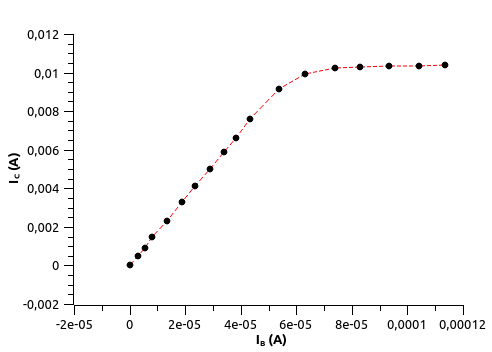
\includegraphics[width=0.8\linewidth]{grafica1}
	\caption{Corriente de colector frente a corriente de base}
	\label{fig:grafica1}
\end{figure}


Se distinguen las tres zonas de trabajo, utilizando $V_{BB}$ como referencia:

\begin{itemize}
	\item \textbf{Zona de corte: } los dos valores por debajo de 0,9 V, en los que la corriente del colector es prácticamente 0.
	\item \textbf{Zona activa: } desde 0,9V hasta 7V, donde la corriente aumenta linealmente.
	\item \textbf{Zona de saturación: } los valores superiores a 7V, en los que la corriente $I_C$ permanece relativamente constante.
\end{itemize}




El voltaje de saturación del transistor es:
\[ V_{CE,SAT} = 0,01 \si{V}
\]

En la Tabla 2 calculamos el valor de $\beta$ para región activa. Elegimos el punto medio.

\begin{table}[H]
	\centering
	\begin{tabular}{|l|l|}
		\hline
		$V_{CE}$  & 3,064 V    \\ \hline
		$V_{BE}$  & 0,647 V   \\ \hline
		$I_C$   & 0,0041 A  \\ \hline
		$I_B$   & 2,35E-05 A\\ \hline
		$\beta$ & 174,25   \\ \hline
	\end{tabular}
	\caption{Valores en punto medio $V_{BB} = 3\si{V}$}
	\label{tab:my-table}
\end{table}



\subsection{Curvas características $I_C - V_{CC}$ para diferentes valores de la corriente de base}

Representamos en las Tablas 3 y 4 los valores para $V_{BB} = 5\si{V}$ y $V_{BB} = 9\si{V}$. En las Figuras 4 y 5 están representadas las $I_C$ frente a $V_{CC}$.



\begin{table}[H]
	\centering
	\begin{tabular}{|l|l|l|l|l|l|}
		\hline
		$V_{CC}$ (V) & $V_{RB}$ (V)   & $I_B$ (A)     & $V_{RC}$ (V)  & $I_C$ (A)    & $V_{CE}$ (V)  \\ 
&[$\pm0,001$] &[$\pm1$E-08] &[$\pm0,001$] &[$\pm2$E-06]  &[$\pm0,001$]\\\hline
		0,3   & 4,34  & 4,34E-05 & 0,268 & 0,00057 & 4,732 \\ \hline
		0,6   & 4,32  & 4,32E-05 & 0,499 & 0,00106 & 4,501 \\ \hline
		0,9   & 4,31  & 4,31E-05 & 0,831 & 0,00177 & 4,169 \\ \hline
		1,2   & 4,34  & 4,34E-05 & 1,153 & 0,00245 & 3,847 \\ \hline
		1,5   & 4,34  & 4,34E-05 & 1,444 & 0,00307 & 3,556 \\ \hline
		2     & 4,33  & 4,33E-05 & 1,853 & 0,00394 & 3,147 \\ \hline
		2,5   & 4,33  & 4,33E-05 & 2,391 & 0,00509 & 2,609 \\ \hline
		3     & 4,32  & 4,32E-05 & 2,785 & 0,00593 & 2,215 \\ \hline
		3,5   & 4,31  & 4,31E-05 & 3,26  & 0,00694 & 1,74  \\ \hline
		4     & 4,32  & 4,32E-05 & 3,44  & 0,00732 & 1,56  \\ \hline
		4,5   & 4,32  & 4,32E-05 & 3,47  & 0,00738 & 1,53  \\ \hline
		5     & 4,32  & 4,32E-05 & 3,5   & 0,00745 & 1,5   \\ \hline
		6     & 4,32  & 4,32E-05 & 3,565 & 0,00759 & 1,435 \\ \hline
		7     & 4,3   & 4,3E-05  & 3,62  & 0,00770 & 1,38  \\ \hline
		8     & 4,32  & 4,32E-05 & 3,67  & 0,00781 & 1,33  \\ \hline
		9     & 4,34  & 4,34E-05 & 3,72  & 0,00791 & 1,28  \\ \hline
		10    & 4,34  & 4,34E-05 & 3,76  & 0,008   & 1,24  \\ \hline
		11    & 4,35  & 4,35E-05 & 3,83  & 0,00815 & 1,17  \\ \hline
		12    & 4,35  & 4,35E-05 & 3,89  & 0,00828 & 1,11  \\ \hline
	\end{tabular}
	\caption{Características para $V_{BB} = 5 \si{V}$}
	\label{tab:my-table}
\end{table}

\begin{table}[H]
	\centering
	\begin{tabular}{|l|l|l|l|l|l|}
		\hline
		$V_{CC}$ (V) & $V_{RB}$ (V)   & $I_B$ (A)     & $V_{RC}$ (V)  & $I_C$ (A)    & $V_{CE}$ (V)  \\ 
&[$\pm0,001$] &[$\pm1$E-08] &[$\pm0,001$] &[$\pm2$E-06]  &[$\pm0,001$]\\\hline
		0,3   & 8,42  & 8,42E-05 & 0,287 & 0,00061 & 4,713 \\ \hline
		0,6   & 8,41  & 8,41E-05 & 0,59  & 0,00126 & 4,41  \\ \hline
		0,9   & 8,4   & 8,4E-05  & 0,85  & 0,00181 & 4,15  \\ \hline
		1,2   & 8,39  & 8,39E-05 & 1,129 & 0,00240 & 3,871 \\ \hline
		1,5   & 8,39  & 8,39E-05 & 1,43  & 0,00304 & 3,57  \\ \hline
		2     & 8,38  & 8,38E-05 & 1,93  & 0,00411 & 3,07  \\ \hline
		2,5   & 8,37  & 8,37E-05 & 2,43  & 0,00517 & 2,57  \\ \hline
		3     & 8,36  & 8,36E-05 & 2,91  & 0,00619 & 2,09  \\ \hline
		3,5   & 8,36  & 8,36E-05 & 3,41  & 0,00726 & 1,59  \\ \hline
		4     & 8,36  & 8,36E-05 & 3,84  & 0,00817 & 1,16  \\ \hline
		4,5   & 8,36  & 8,36E-05 & 4,34  & 0,00923 & 0,66  \\ \hline
		5     & 8,35  & 8,35E-05 & 4,83  & 0,01027 & 0,17  \\ \hline
		6     & 8,35  & 8,35E-05 & 5,67  & 0,01206 & -0,67 \\ \hline
		7     & 8,35  & 8,35E-05 & 6,44  & 0,0137  & -1,44 \\ \hline
		8     & 8,35  & 8,35E-05 & 6,83  & 0,0145  & -1,83 \\ \hline
		9     & 8,36  & 8,36E-05 & 6,95  & 0,0148  & -1,95 \\ \hline
		10    & 8,37  & 8,37E-05 & 7,14  & 0,0152  & -2,14 \\ \hline
		11    & 8,37  & 8,37E-05 & 7,3   & 0,0155  & -2,3  \\ \hline
		12    & 8,38  & 8,38E-05 & 7,41  & 0,0158  & -2,41 \\ \hline
	\end{tabular}
	\caption{Características para $V_{BB} = 9 \si{V}$}
	\label{tab:my-table}
\end{table}

\begin{figure}[H]
	\centering
	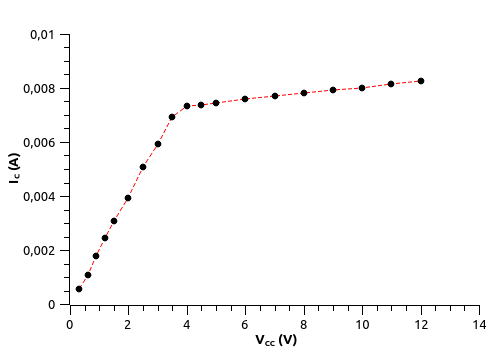
\includegraphics[width=0.8\linewidth]{grafica2}
	\caption{$I_C$ frente a $V_{CC}$ para $V_{BB} = 5\si{V}$}
	\label{fig:grafica2}
\end{figure}

\begin{figure}[H]
	\centering
	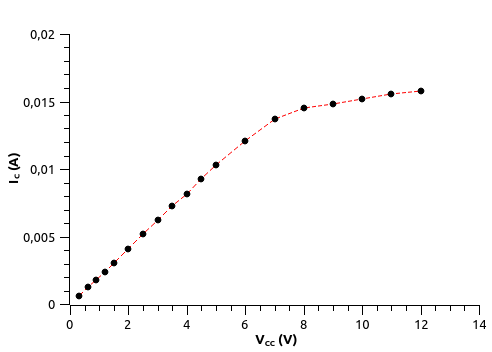
\includegraphics[width=0.8\linewidth]{grafica3}
	\caption{$I_C$ frente a $V_{CC}$ para $V_{BB} = 9\si{V}$}
	\label{fig:grafica3}
\end{figure}

\begin{figure}[H]
	\centering
	\includegraphics[width=0.8\linewidth]{"graficas juntas"}
	\caption{curvas de Figuras 4 y 5 juntas}
	\label{fig:graficas-juntas}
\end{figure}



\subsection{Diferentes circuitos de polarización del transistor}

\subsection*{\textit{Polarización con retroalimentación en base}}

Montamos el circuito de la Figura 7, con los valores de $R_C$ y $R_B$ para obtener el punto de polarización teórico que hemos obtenido en la sección 3.1.


\begin{figure}[H]
	\centering
	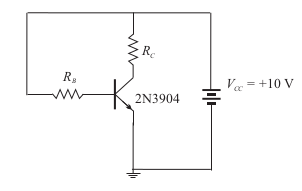
\includegraphics[width=0.7\linewidth]{retroalimentacionenbase}
	\caption{Circuito con retroalimentación en base}
	\label{fig:retroalimentacionenbase}
\end{figure}

\[R_C = \frac{10- V_{CE}}{I_C} = 1683,84 \si{\ohm} \]
\[R_B = \frac{10- V_{BE}}{I_B} = 397492,56\si{\ohm} \]

Las características están recogidas en la Tabla 5.


\begin{table}[H]
	\centering
	\begin{tabular}{|l|l|}
		\hline
		$R_C$  & 1683,84 $\si{\ohm}$  \\ \hline
		$R_B$    & 397492,56   $\si{\ohm}$    \\ \hline
		$V_{RC}$ & 8,73   V   \\ \hline
		$I_C$    & 0,0057  A  \\ \hline
		$V_{RB}$ & 9,43    V  \\ \hline
		$I_B$    & 2,30E-05 A \\ \hline
		$V_{CE}$ & 0,691   V  \\ \hline
	\end{tabular}
	\caption{Características para circuito con retroalimentación en base}
	\label{tab:my-table}
\end{table}

\begin{itemize}
	
	\item¿Qué magnitud se fija con este tipo de polarización? El valor de $I_B$
	
	%Vce, a la mitad de Vcc
	
	\item¿Qué ocurre cuando $\beta$ varía con la temperatura? ¿Cómo de estable es esta polarización frente a variaciones de la temperatura?
	
	No es muy estable, se ve afectada bastante por cambios en la temperatura.
			
\end{itemize}



\subsection*{\textit{Polarización con un divisor de tensión}}

Montamos el circuito de la Figura 8. Obtenemos las resistencias:

\[R_C =  1529,97 \si{\ohm} \]
\[R_B =  2130\si{\ohm} \]


\begin{figure}[H]
	\centering
	\includegraphics[width=0.7\linewidth]{"divisor de tension"}
	\caption{circuito con divisor de tensión}
	\label{fig:divisor-de-tension}
\end{figure}

Las características están en la Tabla 6

\begin{table}[H]
	\centering
	\begin{tabular}{|l|l|}
		\hline
		$R_C$  & 1531 $\si{\ohm}$   \\ \hline
		$R_B$    & 3479 $\si{\ohm}$   \\ \hline
		$V_{RC}$ & 1,47 V   \\ \hline
		$I_C$    & 0,00426 A\\ \hline
		$V_{RB}$ & 1,691  V \\ \hline
		$I_B$     & 9,69 A   \\ \hline
		$V_{CE}$ & 0,691  V \\ \hline
	\end{tabular}
	\caption{Características para circuito con divisor de tensión}
	\label{tab:my-table}
\end{table}

\begin{itemize}
	
	\item¿Qué magnitud se fija con este tipo de polarización? 
	El valor de $I_C$
	\item¿Qué ocurre cuando $\beta$ varía con la temperatura? ¿Cómo de estable es esta polarización frente a variaciones de la temperatura?
	
	Esta configuración es muy estable frente a la temperatura
	
\end{itemize}

\subsection*{\textit{Polarización por realimentación de colector}}

Montamos el circuito de la Figura 9. Obtenemos las resistencias:

\[R_C =  1683,84 \si{\ohm} \]
\[R_B =  102719,93\si{\ohm} \]


\begin{figure}[H]
	\centering
	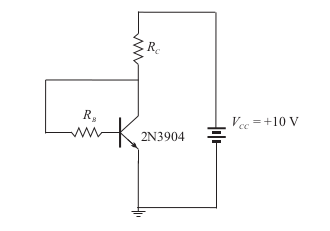
\includegraphics[width=0.7\linewidth]{realimentacioecolector}
	\caption{Circuito con realimentación en colector}
	\label{fig:realimentacioecolector}
\end{figure}


Las características han sido recogidas en la Tabla 7

\begin{table}[H]
	\centering
	\begin{tabular}{|l|l|}
		\hline
		$R_C$  & 1620 $\si{\ohm}$   \\ \hline
		$R_B$    & 100000 $\si{\ohm}$   \\ \hline
		$V_{RC}$ & 7,16 V   \\ \hline
		$I_C$    & 0,003 A\\ \hline
		$V_{RB}$ & 2,87  V \\ \hline
		$I_B$     & 	2,00E-05 A   \\ \hline
		$V_{CE}$ & 2,97  V \\ \hline
	\end{tabular}
	\caption{Características para circuito con realimentación en colector}
	\label{tab:my-table}
\end{table}

\begin{itemize}
	\item¿Cómo se comporta este circuito de polarización con la variación de $\beta$ con la temperatura?
	
	Resulta un tanto más estable que la polarización con retroalimentación en base.
	
\end{itemize}


%%%%%%%%%%%%%%%%%%%%%%%%%%%
\begin{thebibliography}{1}
%%%%%%%%%%%%%%%%%%%%%%%%%%%
	
	
	\bibitem{UNED2022} (varios) Guiones de prácticas- Técnicas Experimentales II. Grado en Física. Versión 2.1  UNED, 2022 \url{https://2022.cursosvirtuales.uned.es/o/3754218}
	%	\bibitem{UNED2021} (varios) Técnicas Experimentales I. Versión 3.5.  UNED, 2021 \url{https://2021.cursosvirtuales.uned.es/o/42035617}
	%\bibitem{2021} Densidad de materiales \url{ https://www.stemm.com/index.php/es/densidades-de-materiales }
	
	
\end{thebibliography}

\end{document}